\documentclass{beamer}
%\includeonlyframes{uj}
\synctex=1
\usepackage[utf8]{inputenc}
\usepackage[ngerman]{babel}
\usepackage[T1]{fontenc}
\usepackage{graphicx}
\usepackage[absolute,overlay]{textpos}
\usepackage{csquotes}
\usepackage{eurosym}
\usepackage{wasysym}
\MakeAutoQuote{„}{”}
\synctex=1
\usepackage{lmodern}

\usepackage{tabularx}
\def\tabularxcolumn#1{m{#1}}

% \usepackage{anyfontsize}


\hypersetup{
  colorlinks=true,
  linkcolor=[rgb]{1, 1, 1}, %
  urlcolor=[rgb]{.2, .2, .5} %
  % allcolors=[rgb]{0, 0, 0} % schwarz
}

\usetheme{Dresden}
\setbeamertemplate{navigation symbols}{}
\setbeamertemplate{footline}[frame number]

\addtobeamertemplate{frametitle}{}{%
  \begin{textblock*}{130mm}(.8\textwidth,8.4mm)
    
\includegraphics[width=4.25cm]{img-src/fsfw-logo.pdf}
  \end{textblock*}
}



\title{Sichere Kommunikation: Warum \& Wie}
\subtitle{KRETA – Oktober 2017}

\begin{document}

\begin{frame}
  \begin{center}
    \begin{tabularx}{7cm}{cc}
      
\includegraphics[width=2.5cm]{img-src/kreta-logo.png}&
      
\includegraphics[width=3cm]{img-src/fsfw-logo-with-text.pdf}\\
      Joschka Heinrich${}^{1}$&
      Carsten Knoll${}^{2}$
    \end{tabularx}

    \vspace*{2\baselineskip}

    \parbox{.95\columnwidth}{\centering\Large\inserttitle}

    \vspace*{\baselineskip}

    \structure{\large \insertsubtitle}

  \end{center}

  ~\\[5mm]
  {\tiny $1$ joschka.heinrich@tu-dresden.de \qquad $2$ casten.knoll@posteo.de}
\end{frame}


%%%%%%%%%%%%%%%%%%%%%%%%%%%%%%%%%%%%%%%%%%%%%%%%%%%%%%%%%%%%%%%%%%%%%%%%%%%%%%%%

\begin{frame}{FSFW – Freie Software und Freies Wissen}

  \begin{columns}

\column[t]{1\textwidth}
\vspace{-5mm}
  \begin{itemize}
  \item Hochschulgruppe seit 2014, ca. 10 Leute (TU, HTW, …)
  \item Warum machen wir das? Aus Überzeugung!

  \begin{itemize}
  \item \emph{Überzeugung 1}: freie und quelloffene Software ist (oft) besser\\
    (technische + nicht technische Argumente)\\
    \bigskip
    \pause
  \item \emph{Überzeugung 2}: öffentlich finanzierte wissenschaftliche Inhalte
    (AutorInnen, GutachterInnen) sollten nicht von öffentlich finanzierten
    Bibliotheken für horrende Summen von Zeitschriften-Verlagen gekauft werden
    müssen
  \end{itemize}

    \pause
  \item Bisherige Projekte
    \begin{itemize}
    \item Linux-Install-Party, Linux-Presentation-Day
    \item Monatliche Sprechstunde zu \LaTeX{} u.a.
    \item Programmpapier
    \item \textbf<4-5>{„Uni-Stick”:~80 $\times$ 8\,GB mit freier Software}
    \item Verschlüsselungsgewinnspiel
    \end{itemize}
    \pause
    \pause
    \pause
    \item Für (Mitmachen-)Interessierte: \url{https://fsfw-dresden.de}
  \end{itemize}

\begin{textblock*}{5cm}[0.,0.](90mm,63mm)
\only<4>{
  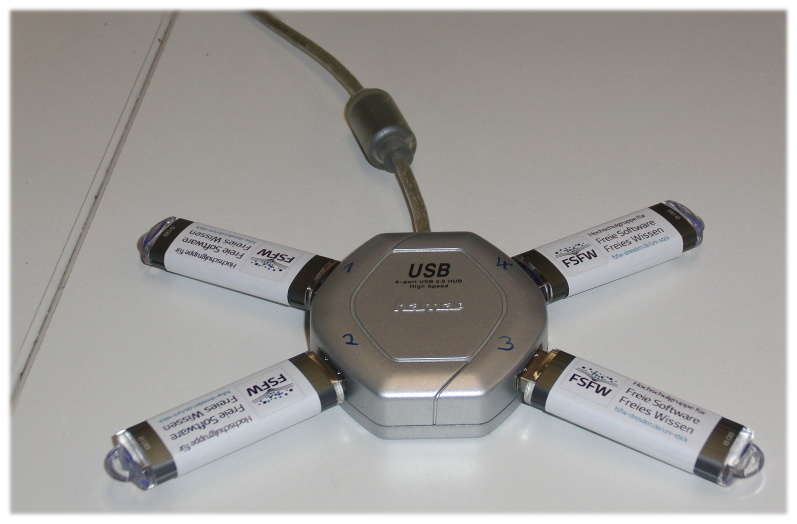
\includegraphics[width=35mm]{img-src/usb-hub}
}
\only<5->{
  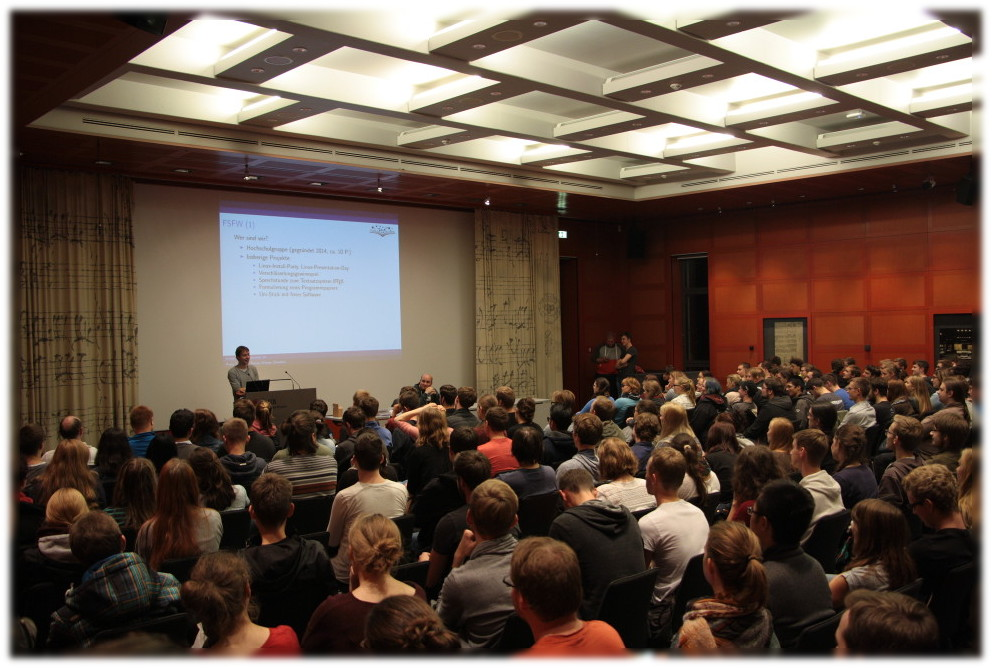
\includegraphics[width=35mm]{img-src/uni-stick-ausgabe-vortrag}
}
\end{textblock*}

\column[t]{.1\textwidth}
~
\end{columns}
\end{frame}

%%%%%%%%%%%%%%%%%%%%%%%%%%%%%%%%%%%%%%%%%%%%%%%%%%%%%%%%%%%%%%%%%%%%%%%%%%%%%%%%

\begin{frame}{Ablauf}

  \textbf{1) Verschlüsselung in der Theorie}
  \begin{itemize}
   \item Diskussion: "`Ich habe doch nichts zu verbergen"'
   \item Schutzziele sicherer Kommunikation
   \item Funktionsweise PGP
  \end{itemize}

  \pause

  \textbf{2) PGP in der Praxis}
  \begin{itemize}
   \item Installation (individuell)
   \item Schlüsselgenerierung
   \item E-Mails verschlüsseln
   \item Ausblick
  \end{itemize}

\end{frame}

%%%%%%%%%%%%%%%%%%%%%%%%%%%%%%%%%%%%%%%%%%%%%%%%%%%%%%%%%%%%%%%%%%%%%%%%%%%%%%%%

\begin{frame}{Diskussion: "`Ich habe doch nichts zu verbergen"'}
  $\rightarrow$ 10 Minuten freie Diskussion

  \begin{itemize}
   \item  je 2-5 Personen
   \item möglichst viele verschiedene Perspektiven einnehmen\\
  (Bürger*in, Bürgerrechtler*in, Innenminister*in, Freiheitskämpfer*in, …)
   \item Argumente sammeln

   \pause

   \item Stichworte
    \begin{itemize}
     \item Kriminalität (Einbruch, Erpressung, …)
     \item Privatsphäre
     \item Selbstzensur (analog: Kamera-Attrappen)
     \item Demokratie
     \item Journalismus
     \item Whistleblowing
     \item Erstarken totalitärer Strukturen
    \end{itemize}
  \end{itemize}

\end{frame}

%%%%%%%%%%%%%%%%%%%%%%%%%%%%%%%%%%%%%%%%%%%%%%%%%%%%%%%%%%%%%%%%%%%%%%%%%%%%%%%

\begin{frame}{"`Ich habe doch nichts zu verbergen"'}

  \begin{itemize}
   \item  In Menschheitsgeschichte:\\
   viele Beispiele für \textbf{rücksichtslosen Egoismus}
   %\item Ausnutzung von Macht zu persönlichem Vorteil
   \item "`Wissen ist Macht"'
   \item[$\Rightarrow$] sensibler Umgang mit Informationen empfehlenswert\\[5mm]

   \pause

   \item \textbf{Digitalisierung verstärkt das Problem}
   \item E-Mail${}^{1}$ ist wie Postkarte: unterwegs${}^{2}$ lesbar
   \item E-Mail ist noch schlimmer als Postkarte:
   \begin{itemize}
    \item automatisiert auswertbar
    \item unbemerkt kopierbar
    \item unbemerkt veränderbar (inkl. Metadaten, bspw. Absender)
   \end{itemize}
  \end{itemize}

  ~\\[5mm]
  {\tiny $1$: E-Mail = nur Beispielmedium \qquad $2$: ggf. um die ganze Welt }

\end{frame}

%%%%%%%%%%%%%%%%%%%%%%%%%%%%%%%%%%%%%%%%%%%%%%%%%%%%%%%%%%%%%%%%%%%%%%%%%%%%%%%%

\begin{frame}{Schutzziele sicherer Kommunikation}

  \begin{itemize}
   \item[$\square$] \textbf{Vertraulichkeit}\\
   $\rightarrow$ A weiß, nur B kann Nachricht lesen

   \pause

   \item[$\square$] \textbf{Integrität}\\
   $\rightarrow$ B weiß, die Nachricht ist nur von A geschrieben und nicht verändert wurden

   \pause

   \item[$\square$] \textbf{Anonymität}\\
   $\rightarrow$ A bestimmt, wem eigene Identität preisgegeben wird

   \pause

   \item[$\square$] \textbf{Verfügbarkeit}\\
   $\rightarrow$ obige Schutzziele werden in annehmbarer Zeit realisiert
  \end{itemize}

\end{frame}

%%%%%%%%%%%%%%%%%%%%%%%%%%%%%%%%%%%%%%%%%%%%%%%%%%%%%%%%%%%%%%%%%%%%%%%%%%%%%%%

\begin{frame}{PGP – Begriffe}

  \begin{columns}
  \column[t]{.48\textwidth}
  \begin{itemize}
   \item asymmetrische Verschlüsselung
   \item Privater Schlüssel\\(\textit{private key})
   \item Öffentlicher Schlüssel\\(\textit{public key})
   \item GPG vs. PGP
  \end{itemize}

  \pause

  \column[t]{.6\textwidth}
  \begin{itemize}
   \item Schlüsselserver (\textit{keyserver})
   \item Fingerabdruck
   \item Metadaten
   \item Widerrufszertifikat
  \end{itemize}
\end{columns}
\end{frame}

%%%%%%%%%%%%%%%%%%%%%%%%%%%%%%%%%%%%%%%%%%%%%%%%%%%%%%%%%%%%%%%%%%%%%%%%%%%%%%%%

\begin{frame}{PGP – Das Problem}

  \begin{itemize}
   \item \textit{P1:} A möchte Nachricht an B vertraulich schicken\\
   \item[$\Rightarrow$] Nachricht verschlüsseln

   \pause

   \vspace*{.5\baselineskip}

   \item\textit{P2:} Schlüsselverteilung\\
   \item[$\Rightarrow$] asymmetrisches Verschlüsselungsverfahren (\texttt{PGP})
   \begin{itemize}
    \item Es gibt: \textbf{ö}ffentlicher \textbf{S}chlüssel und \textbf{p}rivater \textbf{S}chlüssel
    %\item sehr große zufällige Zahlen (dargestellt als \href{https://cknoll.github.io/files/pub-key-carsten.txt}{Zeichen}\href{file:///home/ck/pub-key-carsten-demo.txt}{salat})

    \pause

    \vspace*{.5\baselineskip}

    \item \textbf{ÖS}: zum Verschlüsseln\\
    {\vspace*{4mm}\hspace{12mm}
\includegraphics[width=7mm]{img-src/padlock-lock}}


    \item \textbf{PS}: zum Entschlüsseln\\
    {\vspace*{4mm}\hspace{5mm}
\includegraphics[width=14mm]{img-src/padlock-unlock-with-key}}

   \end{itemize}
  \end{itemize}

  \pause

  {\tiny Oft eingesetzte, freie Implementierung: \texttt{GPG} (\textbf{G}NU \textbf{P}rivacy \textbf{G}uard, 1999)\\
  Nicht freier Vorläufer \& Namensgeber des Verfahrens: \texttt{PGP} (\textbf{P}retty \textbf{G}ood \textbf{P}rivacy, 1991)}

% padlock: <div>Icons made by <a href="http://www.flaticon.com/authors/dave-gandy" title="Dave Gandy">Dave Gandy</a> from <a href="http://www.flaticon.com" title="Flaticon">www.flaticon.com</a> is licensed by <a href="http://creativecommons.org/licenses/by/3.0/" title="Creative Commons BY 3.0" target="_blank">CC 3.0 BY</a></div>
% key: <div>Icons made by <a href="http://www.flaticon.com/authors/yannick" title="Yannick">Yannick</a> from <a href="http://www.flaticon.com" title="Flaticon">www.flaticon.com</a> is licensed by <a href="http://creativecommons.org/licenses/by/3.0/" title="Creative Commons BY 3.0" target="_blank">CC 3.0 BY</a></div>

\end{frame}

%%%%%%%%%%%%%%%%%%%%%%%%%%%%%%%%%%%%%%%%%%%%%%%%%%%%%%%%%%%%%%%%%%%%%%%%%%%%%%%

\begin{frame}{PGP – Funktionsweise 1}

\begin{center}
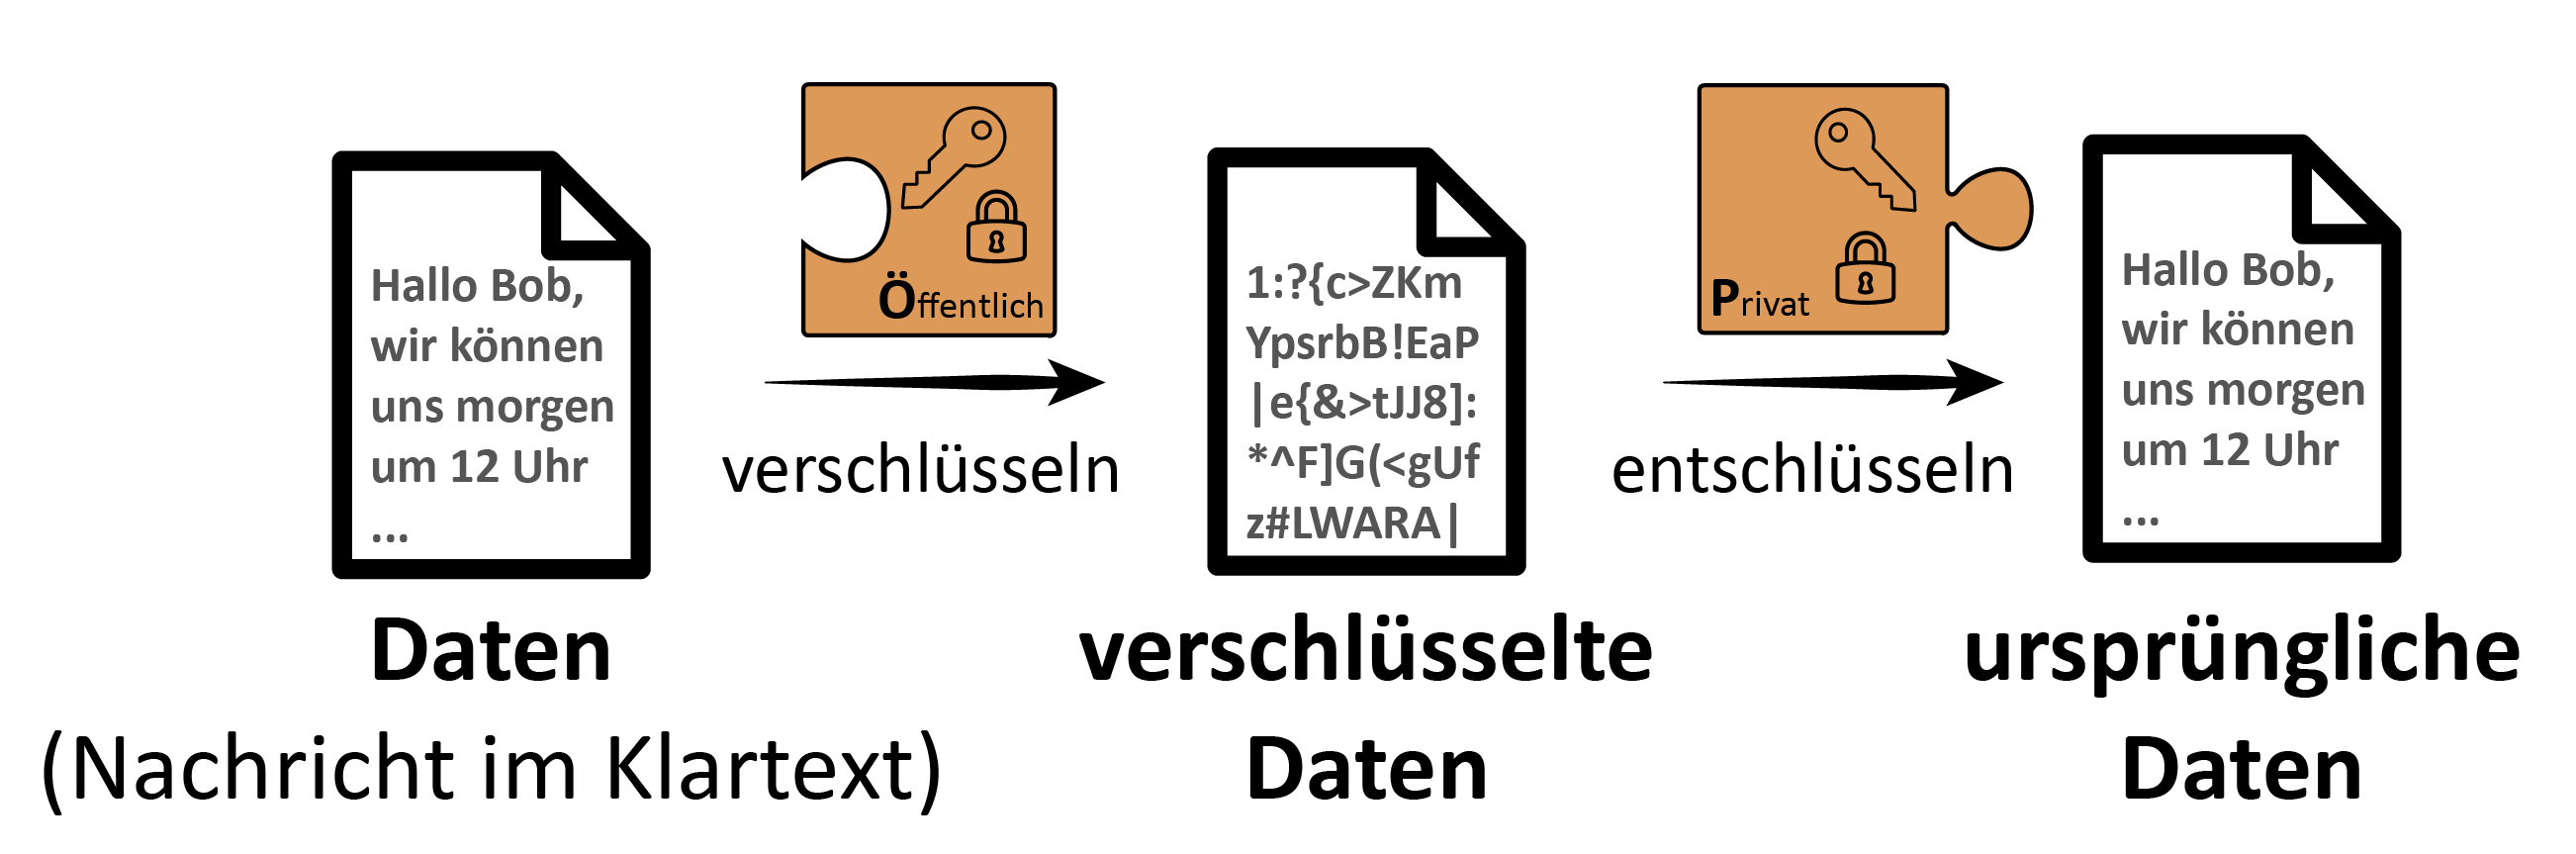
\includegraphics[width=\textwidth]{img-src/pgp_ver_entschluesseln.png}
\end{center}
\end{frame}

%%%%%%%%%%%%%%%%%%%%%%%%%%%%%%%%%%%%%%%%%%%%%%%%%%%%%%%%%%%%%%%%%%%%%%%%%%%%%%%

\begin{frame}{PGP – Funktionsweise 2}

    \begin{itemize}
   \item Öffentlicher Schlüssel ("`public key"')
   \begin{itemize}
    \item Benötigt zum Verschlüsseln
    \item Sollten alle haben, von denen man verschlüsselte Mails empfangen möchte
    \item kann/sollte man weitergeben $\rightarrow$ auf Keyserver hochladen\\
    {\tiny Bsp: \url{http://pgp.mit.edu} \quad zu bedenken: nicht löschbar, nur widerrufbar $\Rightarrow$ Anonymität gefährdet}

   \end{itemize}
   \pause
   \item Privater Schlüssel ("`private key"')
   \begin{itemize}
    \item Benötigt zum Entschlüsseln
    \item Darf nicht verloren gehen\\$\rightarrow$ Entschlüsseln wäre dann unmöglich\\[1mm]
    \item Darf nicht in fremde Hände kommen\\ $\rightarrow$ andere können meine Mails entschlüsseln\\[1mm]
    \item Typischerweise nochmal zusätzlich mit einem Passwort verschlüsselt\\[2mm]
    \pause
    \item[$\Rightarrow$] Sicheres Backup wichtig
   \end{itemize}


  \end{itemize}

\end{frame}

%%%%%%%%%%%%%%%%%%%%%%%%%%%%%%%%%%%%%%%%%%%%%%%%%%%%%%%%%%%%%%%%%%%%%%%%%%%%%%%

\begin{frame}{PGP – Funktionsweise 3}
\begin{center}
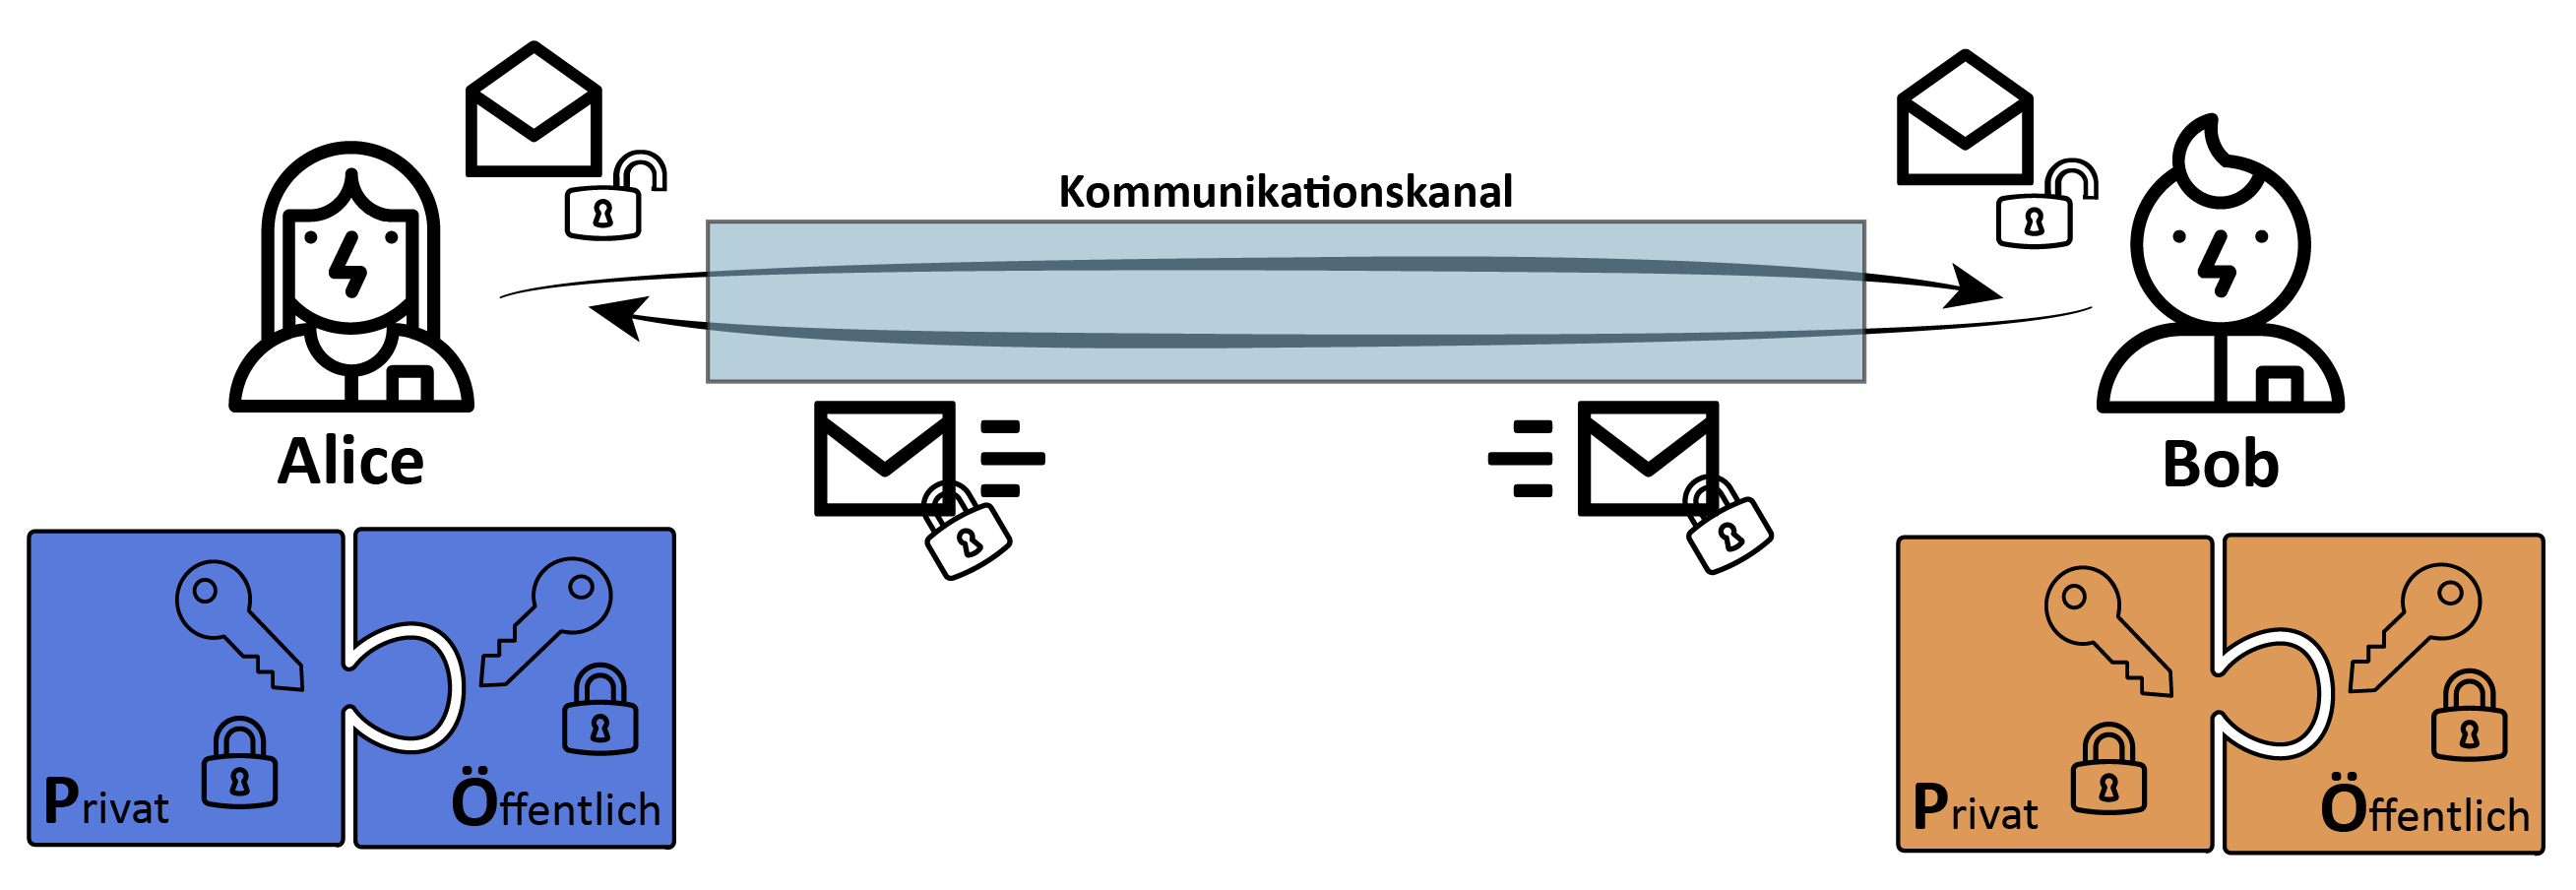
\includegraphics[width=\textwidth]{img-src/pgp_kommunikationskanal.png}
\end{center}
\end{frame}

%%%%%%%%%%%%%%%%%%%%%%%%%%%%%%%%%%%%%%%%%%%%%%%%%%%%%%%%%%%%%%%%%%%%%%%%%%%%%%%%

\begin{frame}{Praxisteil – Installation 1}

  \begin{center}
  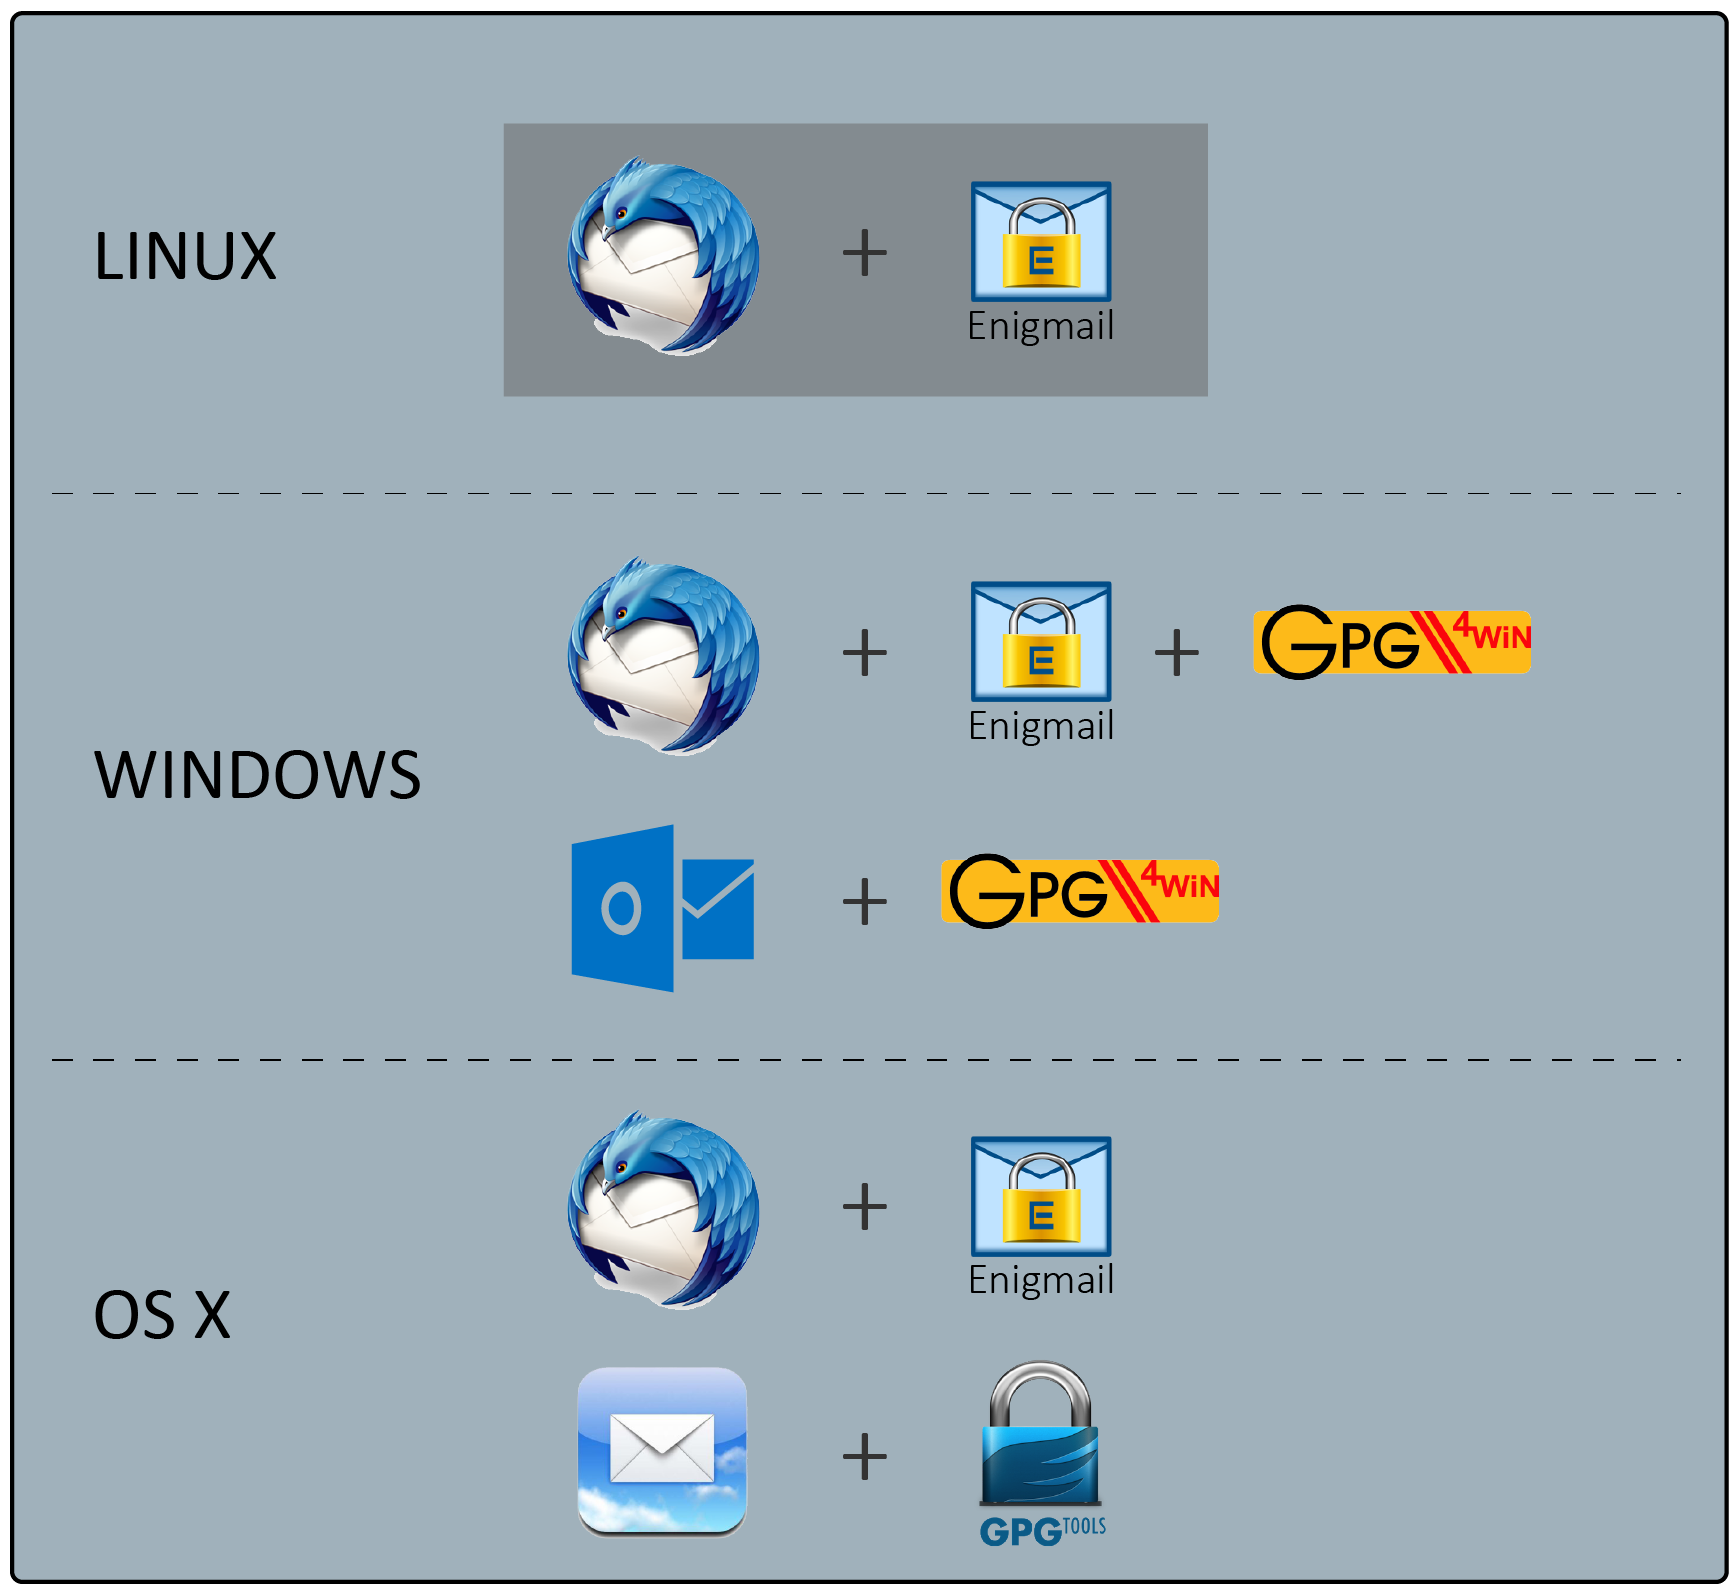
\includegraphics[width=.6\textwidth]{img-src/pgp_software.png}
  \end{center}

  \begin{itemize}
    \item Anleitungen: \url{https://fsfw-dresden.de/gpg}
  \end{itemize}

\end{frame}

%%%%%%%%%%%%%%%%%%%%%%%%%%%%%%%%%%%%%%%%%%%%%%%%%%%%%%%%%%%%%%%%%%%%%%%%%%%%%%%%

\begin{frame}{Praxisteil – Installation 2}
  \begin{itemize}
  \item Anleitungen: \url{https://fsfw-dresden.de/gpg}
  \item temporäre E-Mailadressen zum Test:
  \begin{itemize}
    \item Adresse/User: \texttt{pgp-test-0$x$@hejn.de} ($x = 1 .. 5$)
    \item Mailserver: \texttt{vega.uberspace.de}
    \item IMAP, Port: 993
    \item Passwort: \texttt{fingerprint}
  \end{itemize}
  \end{itemize}
\end{frame}

%%%%%%%%%%%%%%%%%%%%%%%%%%%%%%%%%%%%%%%%%%%%%%%%%%%%%%%%%%%%%%%%%%%%%%%%%%%%%%%%

\begin{frame}{Schlüsselgenerierung}
  \begin{center}
  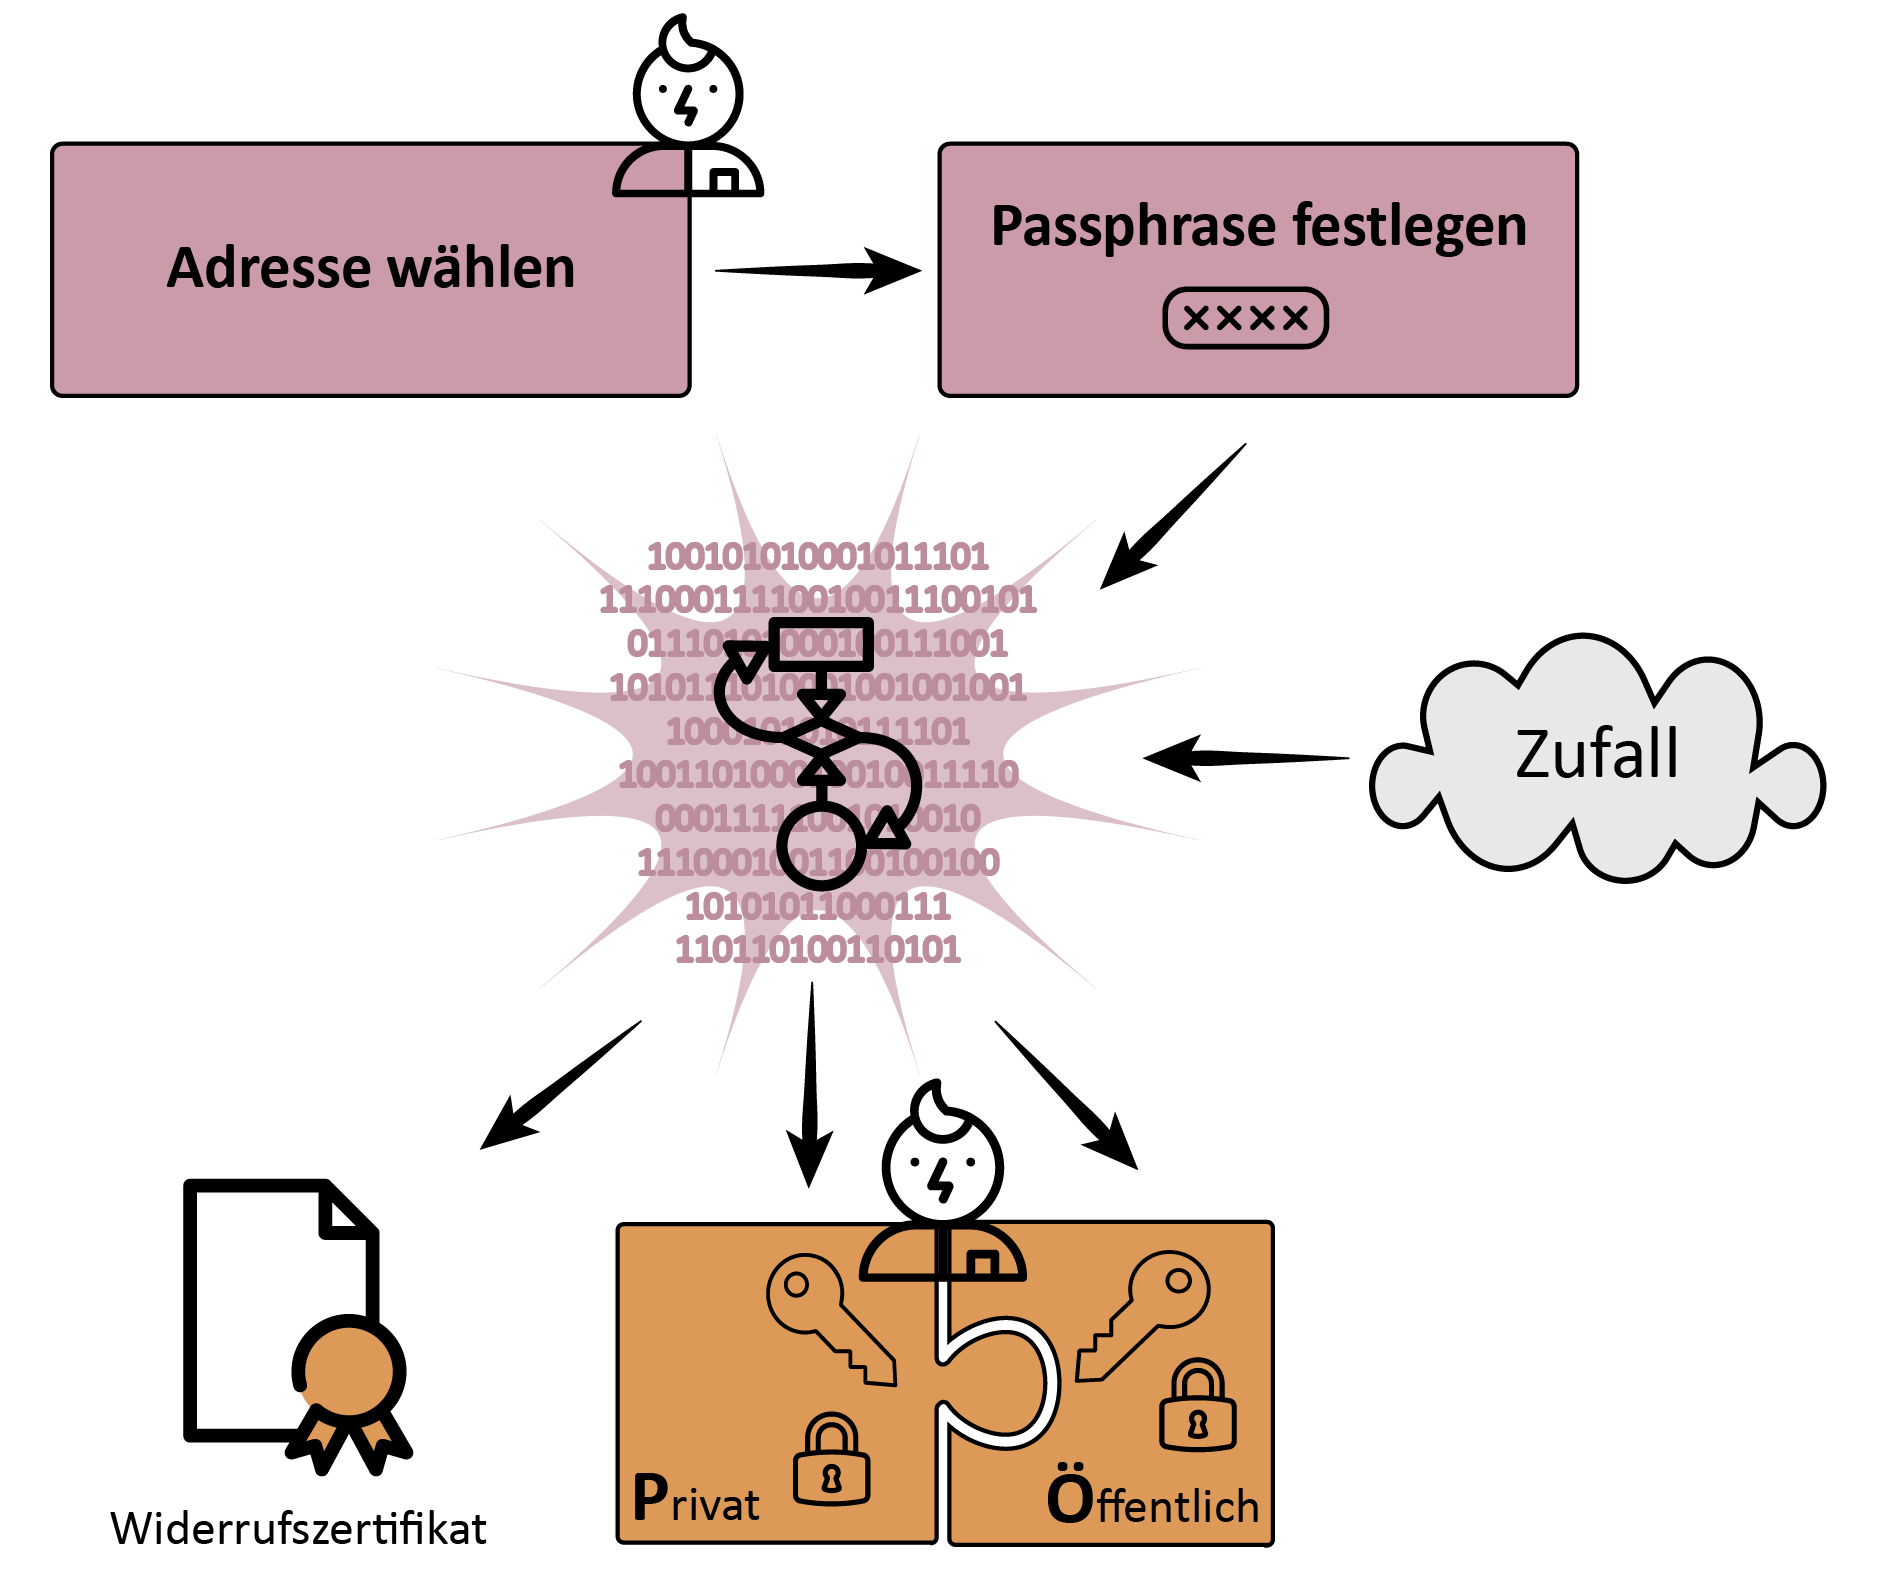
\includegraphics[width=.8\textwidth]{img-src/pgp_keygen.png}
  \end{center}
\end{frame}

%%%%%%%%%%%%%%%%%%%%%%%%%%%%%%%%%%%%%%%%%%%%%%%%%%%%%%%%%%%%%%%%%%%%%%%%%%%%%%%%

\begin{frame}{E-Mails verschlüsseln}

  $\rightarrow$ ÖS müssen bereits ausgetauscht sein!

  \begin{center}
  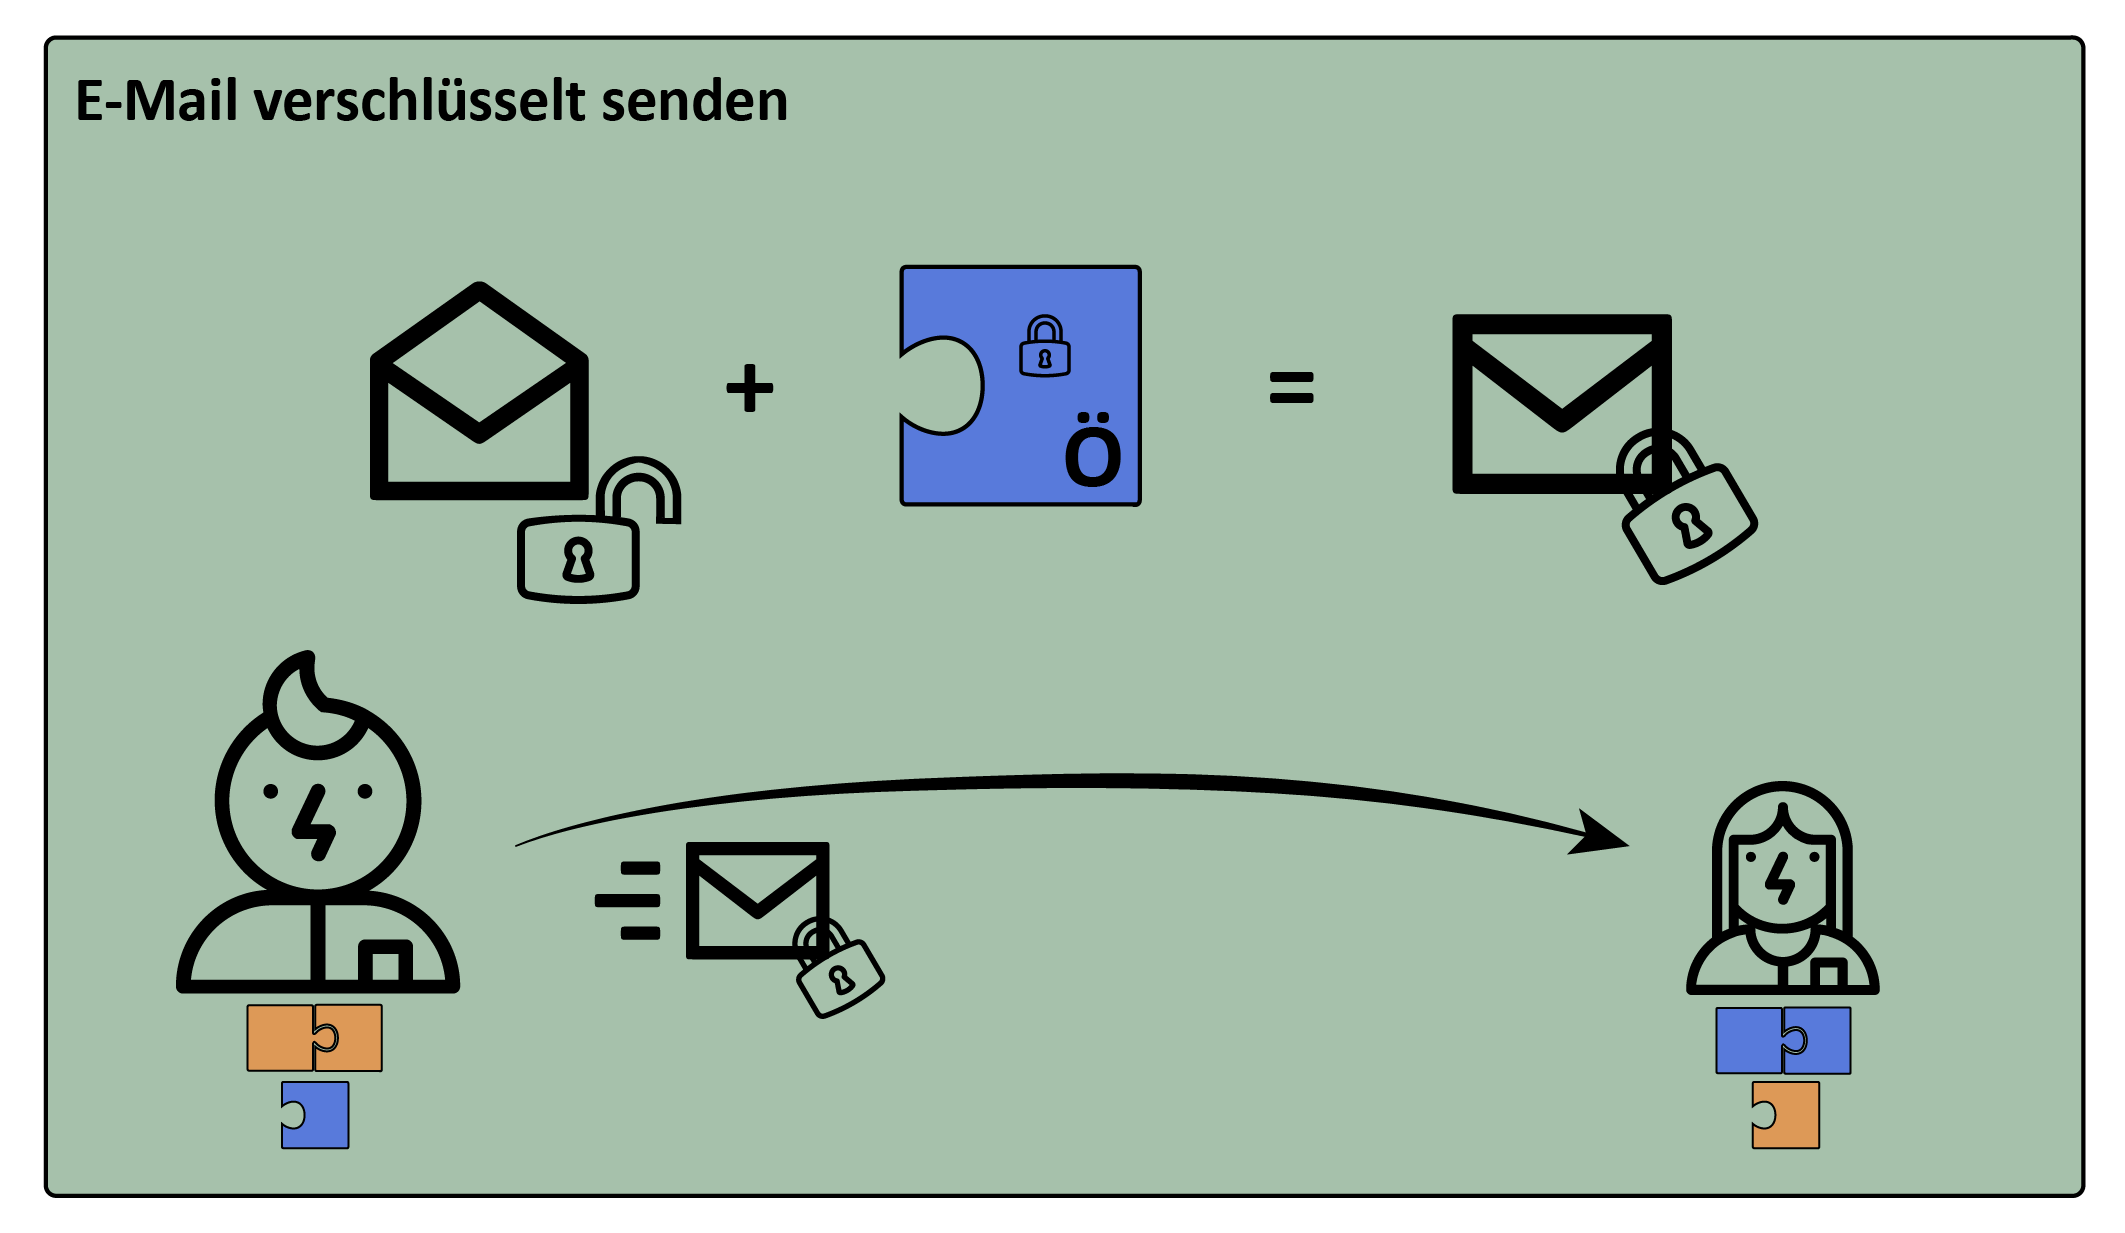
\includegraphics[width=.9\textwidth]{img-src/pgp_enc.png}
  \end{center}

  Testmail (mit Schlüssel im Anhang) an: \texttt{vertraulich@hejn.de}

\end{frame}

%%%%%%%%%%%%%%%%%%%%%%%%%%%%%%%%%%%%%%%%%%%%%%%%%%%%%%%%%%%%%%%%%%%%%%%%%%%%%%%%

\begin{frame}{E-Mails entschlüsseln}
  \begin{center}
  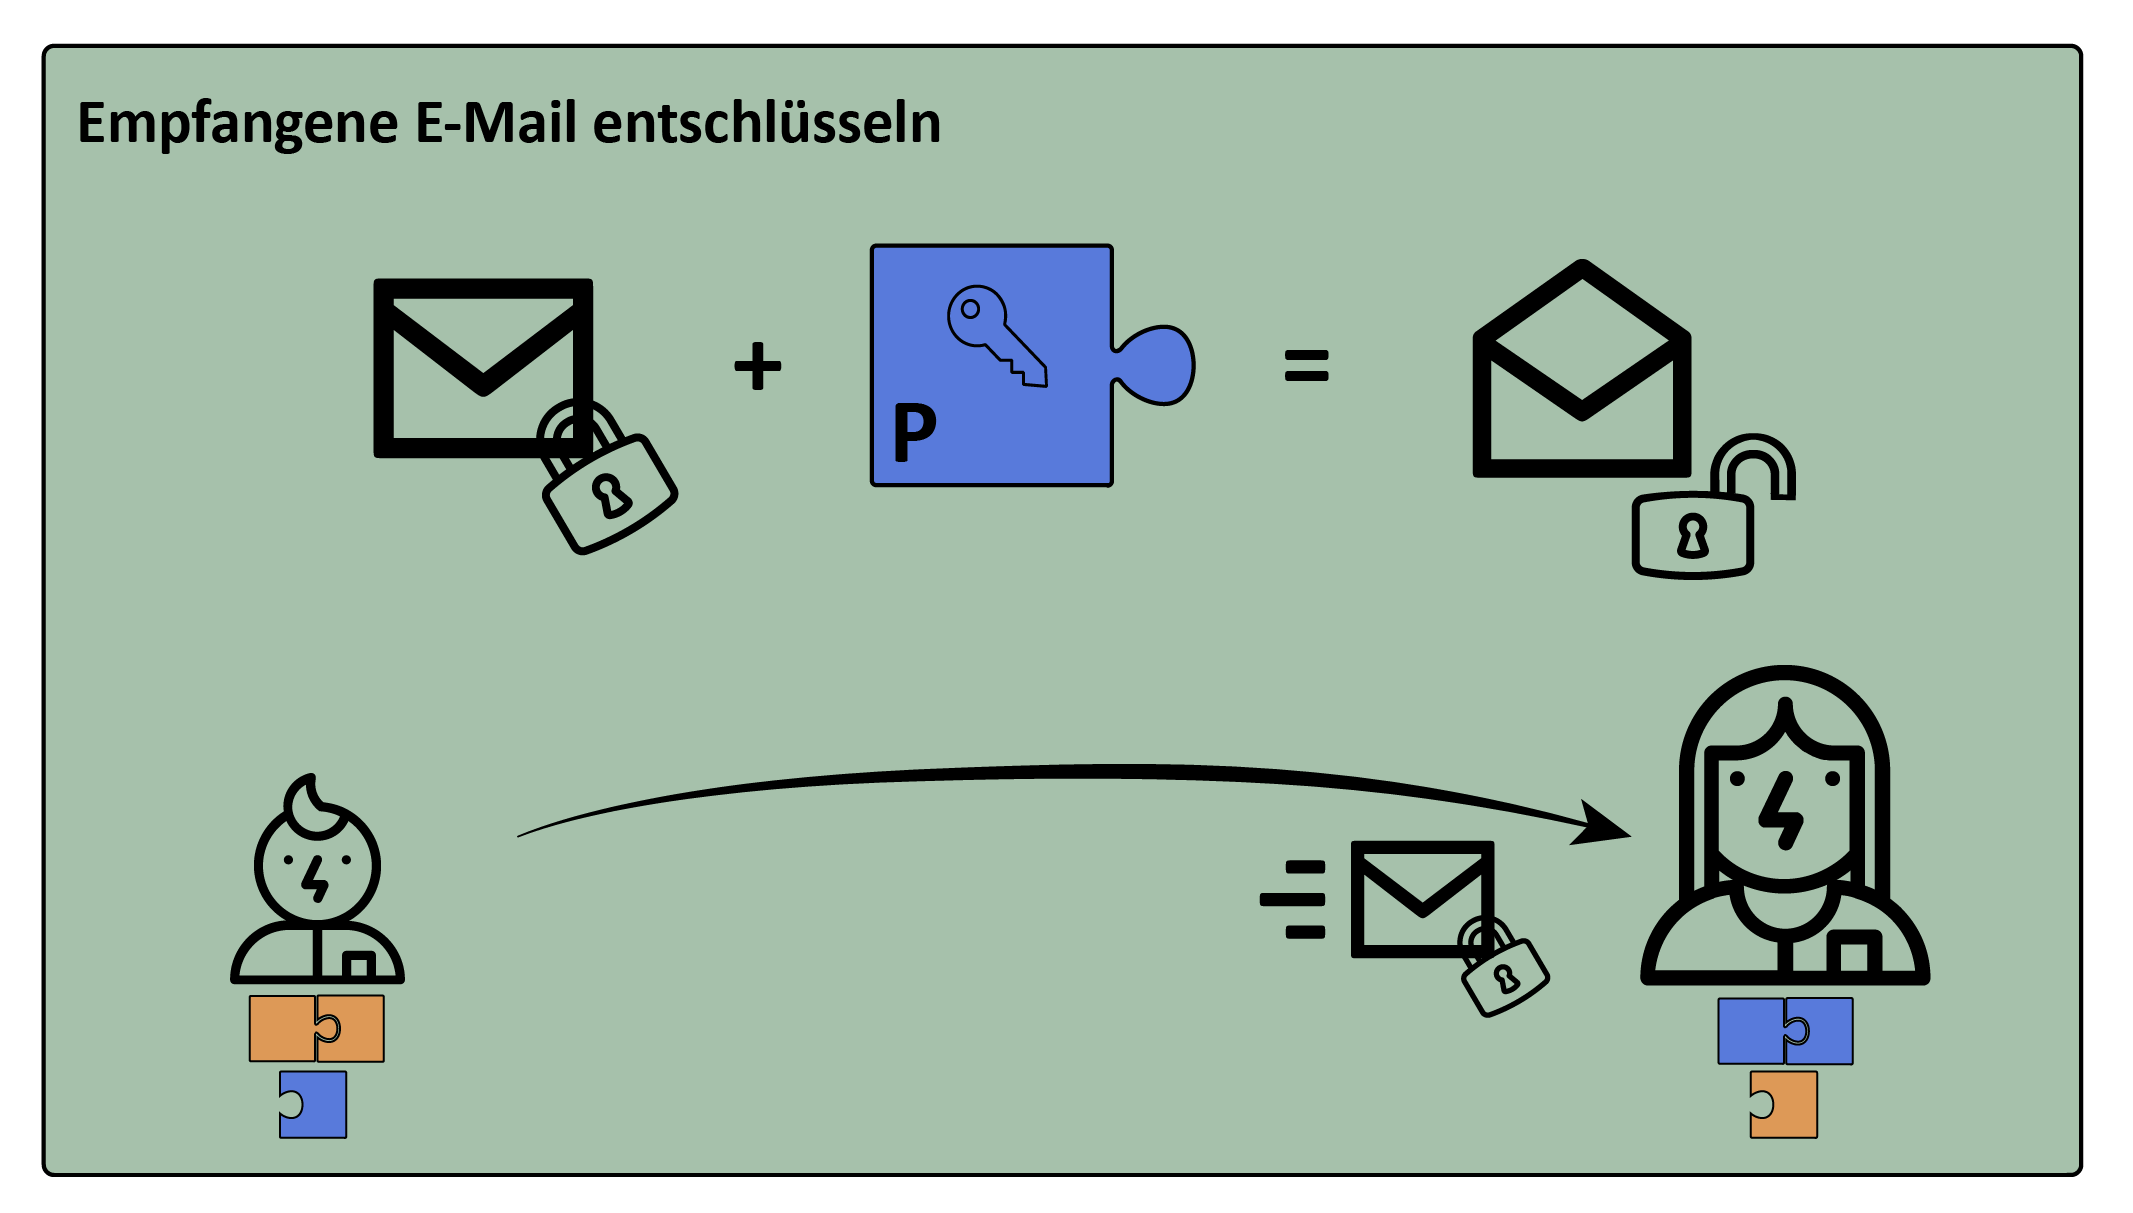
\includegraphics[width=.9\textwidth]{img-src/pgp_dec.png}
  \end{center}
\end{frame}

%%%%%%%%%%%%%%%%%%%%%%%%%%%%%%%%%%%%%%%%%%%%%%%%%%%%%%%%%%%%%%%%%%%%%%%%%%%%%%%

 \begin{frame}{Ausblick – Schutzziele bei PGP}
  \begin{itemize}
   \item[$\square$\visible<2->{\hspace{-.67em}\raisebox{0.1em}{\scalebox{1.3}{\checkmark}}}] Vertraulichkeit \visible<2->{$\rightarrow$ Verschlüsselung}

   \item[$\square$\scalebox{1.25}{~}] Integrität (keine Veränderung) \visible<3->{$\rightarrow$ Signatur notwendig}

   \item[$\square$\scalebox{1.25}{~}] Anonymität

   \item[$\square$\visible<4->{\hspace{-.67em}\raisebox{0.1em}{\scalebox{1.3}{\checkmark}}}] Verfügbarkeit
  \end{itemize}
  \pause
  \pause
  \pause

\end{frame}

%%%%%%%%%%%%%%%%%%%%%%%%%%%%%%%%%%%%%%%%%%%%%%%%%%%%%%%%%%%%%%%%%%%%%%%%%%%%%%%

\begin{frame}{Ausblick – Signieren 1}

  \begin{itemize}
   \item Prinzip: mit PS verschlüsselte Prüfsumme der Nachricht
   \item Überprüfen $=$ Entschlüsseln mit ÖS
   \item[$\Rightarrow$] Man muss dem öffentlichen Schlüssel vertrauen\\[2mm]
   \item[$\square$\hspace{-.67em}\raisebox{0.1em}{\scalebox{1.3}{\checkmark}}] Integrität (keine Veränderung)
   \pause

   \item Schlüssel signieren bei persönlichem Treffen (Keysharing-Party) $\rightarrow$ "`Web of trust"'
   \item Fingerabdruck-Bsp:\\
   \texttt{214E 4E9D B193 6AF2 CFDC 68DF 13AD 3604 \textbf{9D3E F6BF}}
  \end{itemize}

\end{frame}

%%%%%%%%%%%%%%%%%%%%%%%%%%%%%%%%%%%%%%%%%%%%%%%%%%%%%%%%%%%%%%%%%%%%%%%%%%%%%%%%

\begin{frame}{Ausblick – Signieren 2}
  \begin{center}
  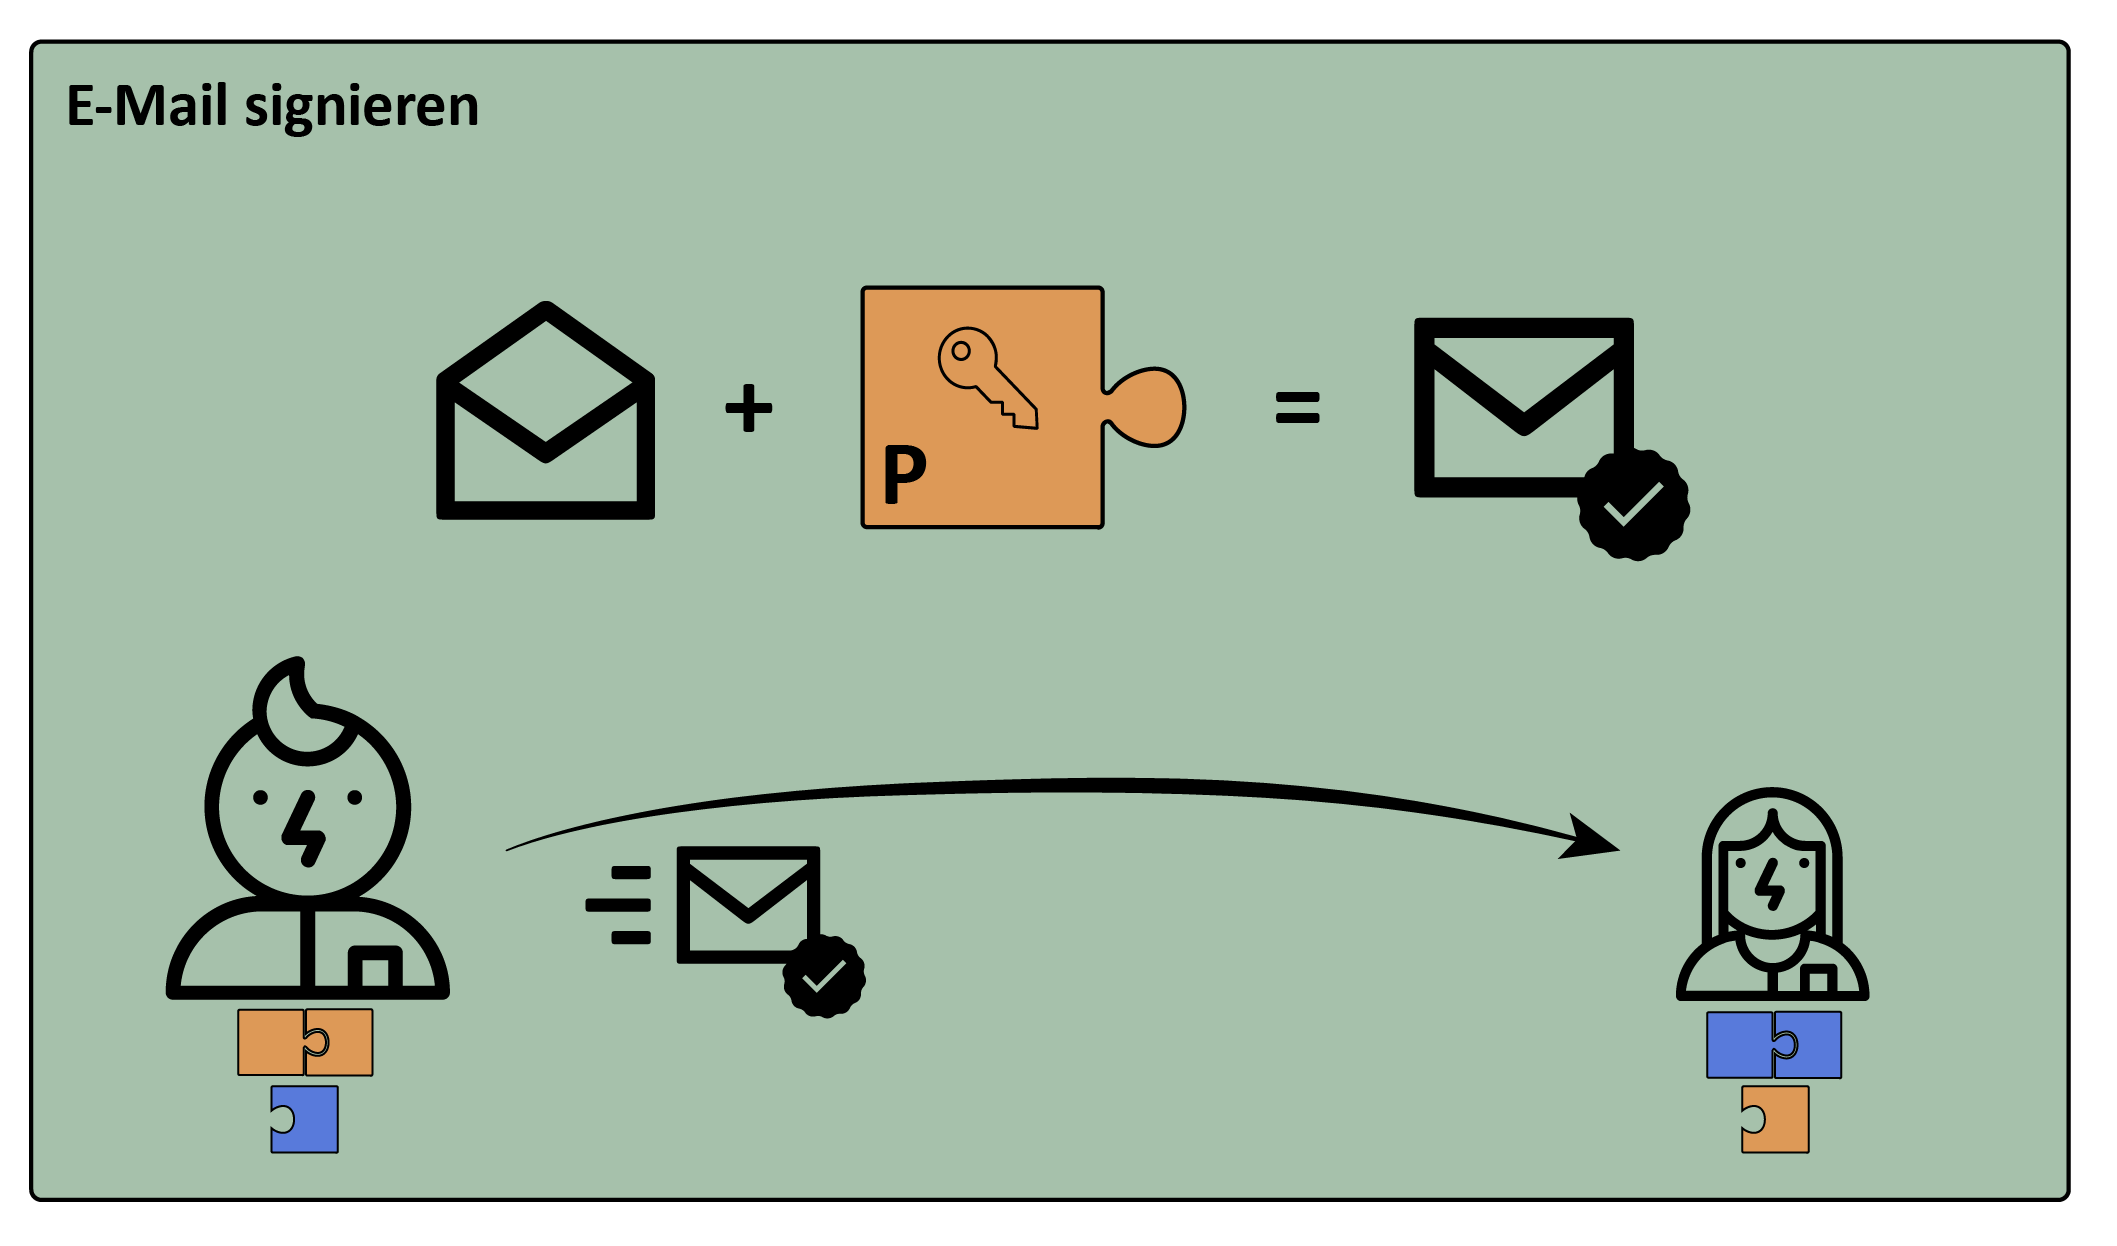
\includegraphics[width=.9\textwidth]{img-src/pgp_sig.png}
  \end{center}
\end{frame}

%%%%%%%%%%%%%%%%%%%%%%%%%%%%%%%%%%%%%%%%%%%%%%%%%%%%%%%%%%%%%%%%%%%%%%%%%%%%%%%

\begin{frame}{Ausblick – Schlüssel pflegen}
  \begin{itemize}
  \item Ablaufdatum $\Rightarrow$ Verlängerung notwendig!
  \begin{itemize}
    \item[$\rightarrow$] ggf. neu auf Schlüsselserver hochladen!
  \end{itemize}

  \pause
  \vspace*{\baselineskip}

  \item Widerrufszertifikat sichern
  \begin{itemize}
    \item[$\rightarrow$] wir benötigt falls:
    \begin{itemize}
      \item Passphrase vergessen
      \item PS verloren ($\rightarrow$ Backup!)
      \item Vertrauen in PS verloren
    \end{itemize}
  \end{itemize}
  \end{itemize}
\end{frame}

%%%%%%%%%%%%%%%%%%%%%%%%%%%%%%%%%%%%%%%%%%%%%%%%%%%%%%%%%%%%%%%%%%%%%%%%%%%%%%%

\begin{frame}{Ausblick – Nachteile PGP}
Was wird verschlüsselt?
\begin{itemize}
\item Text
\item Anhänge {\tiny Format-Empfehlung: \texttt{PGP/MIME} \quad nicht: \texttt{Inline PGP}}
\item[]
\end{itemize}
Was wird nicht verschlüsselt?
\begin{itemize}
 \item Metadaten
 \begin{itemize}
  \item Absender*in, Empfänger*in, \textbf{Betreff}, …
  \item[]
 \end{itemize}
\end{itemize}
\end{frame}

%%%%%%%%%%%%%%%%%%%%%%%%%%%%%%%%%%%%%%%%%%%%%%%%%%%%%%%%%%%%%%%%%%%%%%%%%%%%%%%%

\begin{frame}{Weitereführendes (1)}

\begin{itemize}
 \item Datenspuren (21. - 22. Okt.)\\[-6mm]
\url{https://www.datenspuren.de}
\hspace{12mm}\raisebox{-1mm}{
\includegraphics[width=2cm]{img-src/datenspuren}}
   \begin{itemize}
   \item Öffentliches Symposium des \href{CCC Dresden}{http://c3d2.de/}
   \item Vorträge, Info-Stände, Workshops u.v.m.

   \end{itemize}
   \item[]
   \item Umundu-Festival (20. - 28. Okt.)
   \begin{itemize}
    \item Festival für nachhaltige Entwicklung
    \item Fokus Thema 2017: Armut und Reichtum
    \item Filme, Vorträge, Workshops, ...
    \item \url{https://umundu.de/}
   \end{itemize}
\end{itemize}


\begin{textblock*}{2cm}[0.,0.](90mm,53mm)
\includegraphics[width=2cm]{img-src/umundu-postkarte}
\end{textblock*}

\end{frame}



\begin{frame}{Weitereführendes (2)}

\begin{itemize}
\item[] \hspace{-2em} PGP-Verschlüsselung für Webmail
  \item \url{https://vimeo.com/178702500} (Screencast)\\[2mm]
  \item \href{https://posteo.de/hilfe/wie-installiere-ich-eine-ende-zu-ende-verschluesselung-pgp-im-browser}{Anleitung von Posteo}
  \item[] \hspace{-2em} Allgemeine Infos
  \item \url{https://virtual-privacy.org}
  \item[] \hspace{-2em} Cryptopartys
  \item \url{https://www.cryptoparty.in}
  \item \url{https://de.wikipedia.org/wiki/CryptoParty}
  \item[] \hspace{-2em} Radio
  \item \href{http://www.deutschlandfunk.de/ein-essay-ueber-geheimnisse-niemand-hat-nichts-zu-verbergen.1184.de.html?dram:article_id=395252}{Deutschlandfunk-Essay: \textit{Niemand hat nichts zu verbergen}}
  \item[] \hspace{-2em} Videos
  \item \href{https://www.ted.com/talks/glenn_greenwald_why_privacy_matters}{G. Greenwald: \textit{Why privacy matters}}
  \item \href{https://www.youtube.com/watch?v=XEVlyP4_11M}{J. Oliver + E. Snwoden (lustig)}
\end{itemize}
\end{frame}

\end{document}